\documentclass[11pt]{article}
\usepackage{graphicx}
\usepackage{float}

\begin{document}

\title{The Crane Problem}
\author{Ivan Almer and Mislav Krstulović}

\maketitle

\section{Problem Statement}

\subsection{Backstory}
On a sunny day in Cartagena (Spain) my friend Mislav and me were chilling on the rooftop of our apartment overlooking the nearby mountains. Next to us there was a moving crane which led us to a discussion whether it is possible that, looking at the crane from above, the load carried by the crane always has the linear path from some starting point to its destination.
This motivated us to further define the problem and already seemed like it had potential for some mental gymnastics.

\begin{figure}[H]
\centering
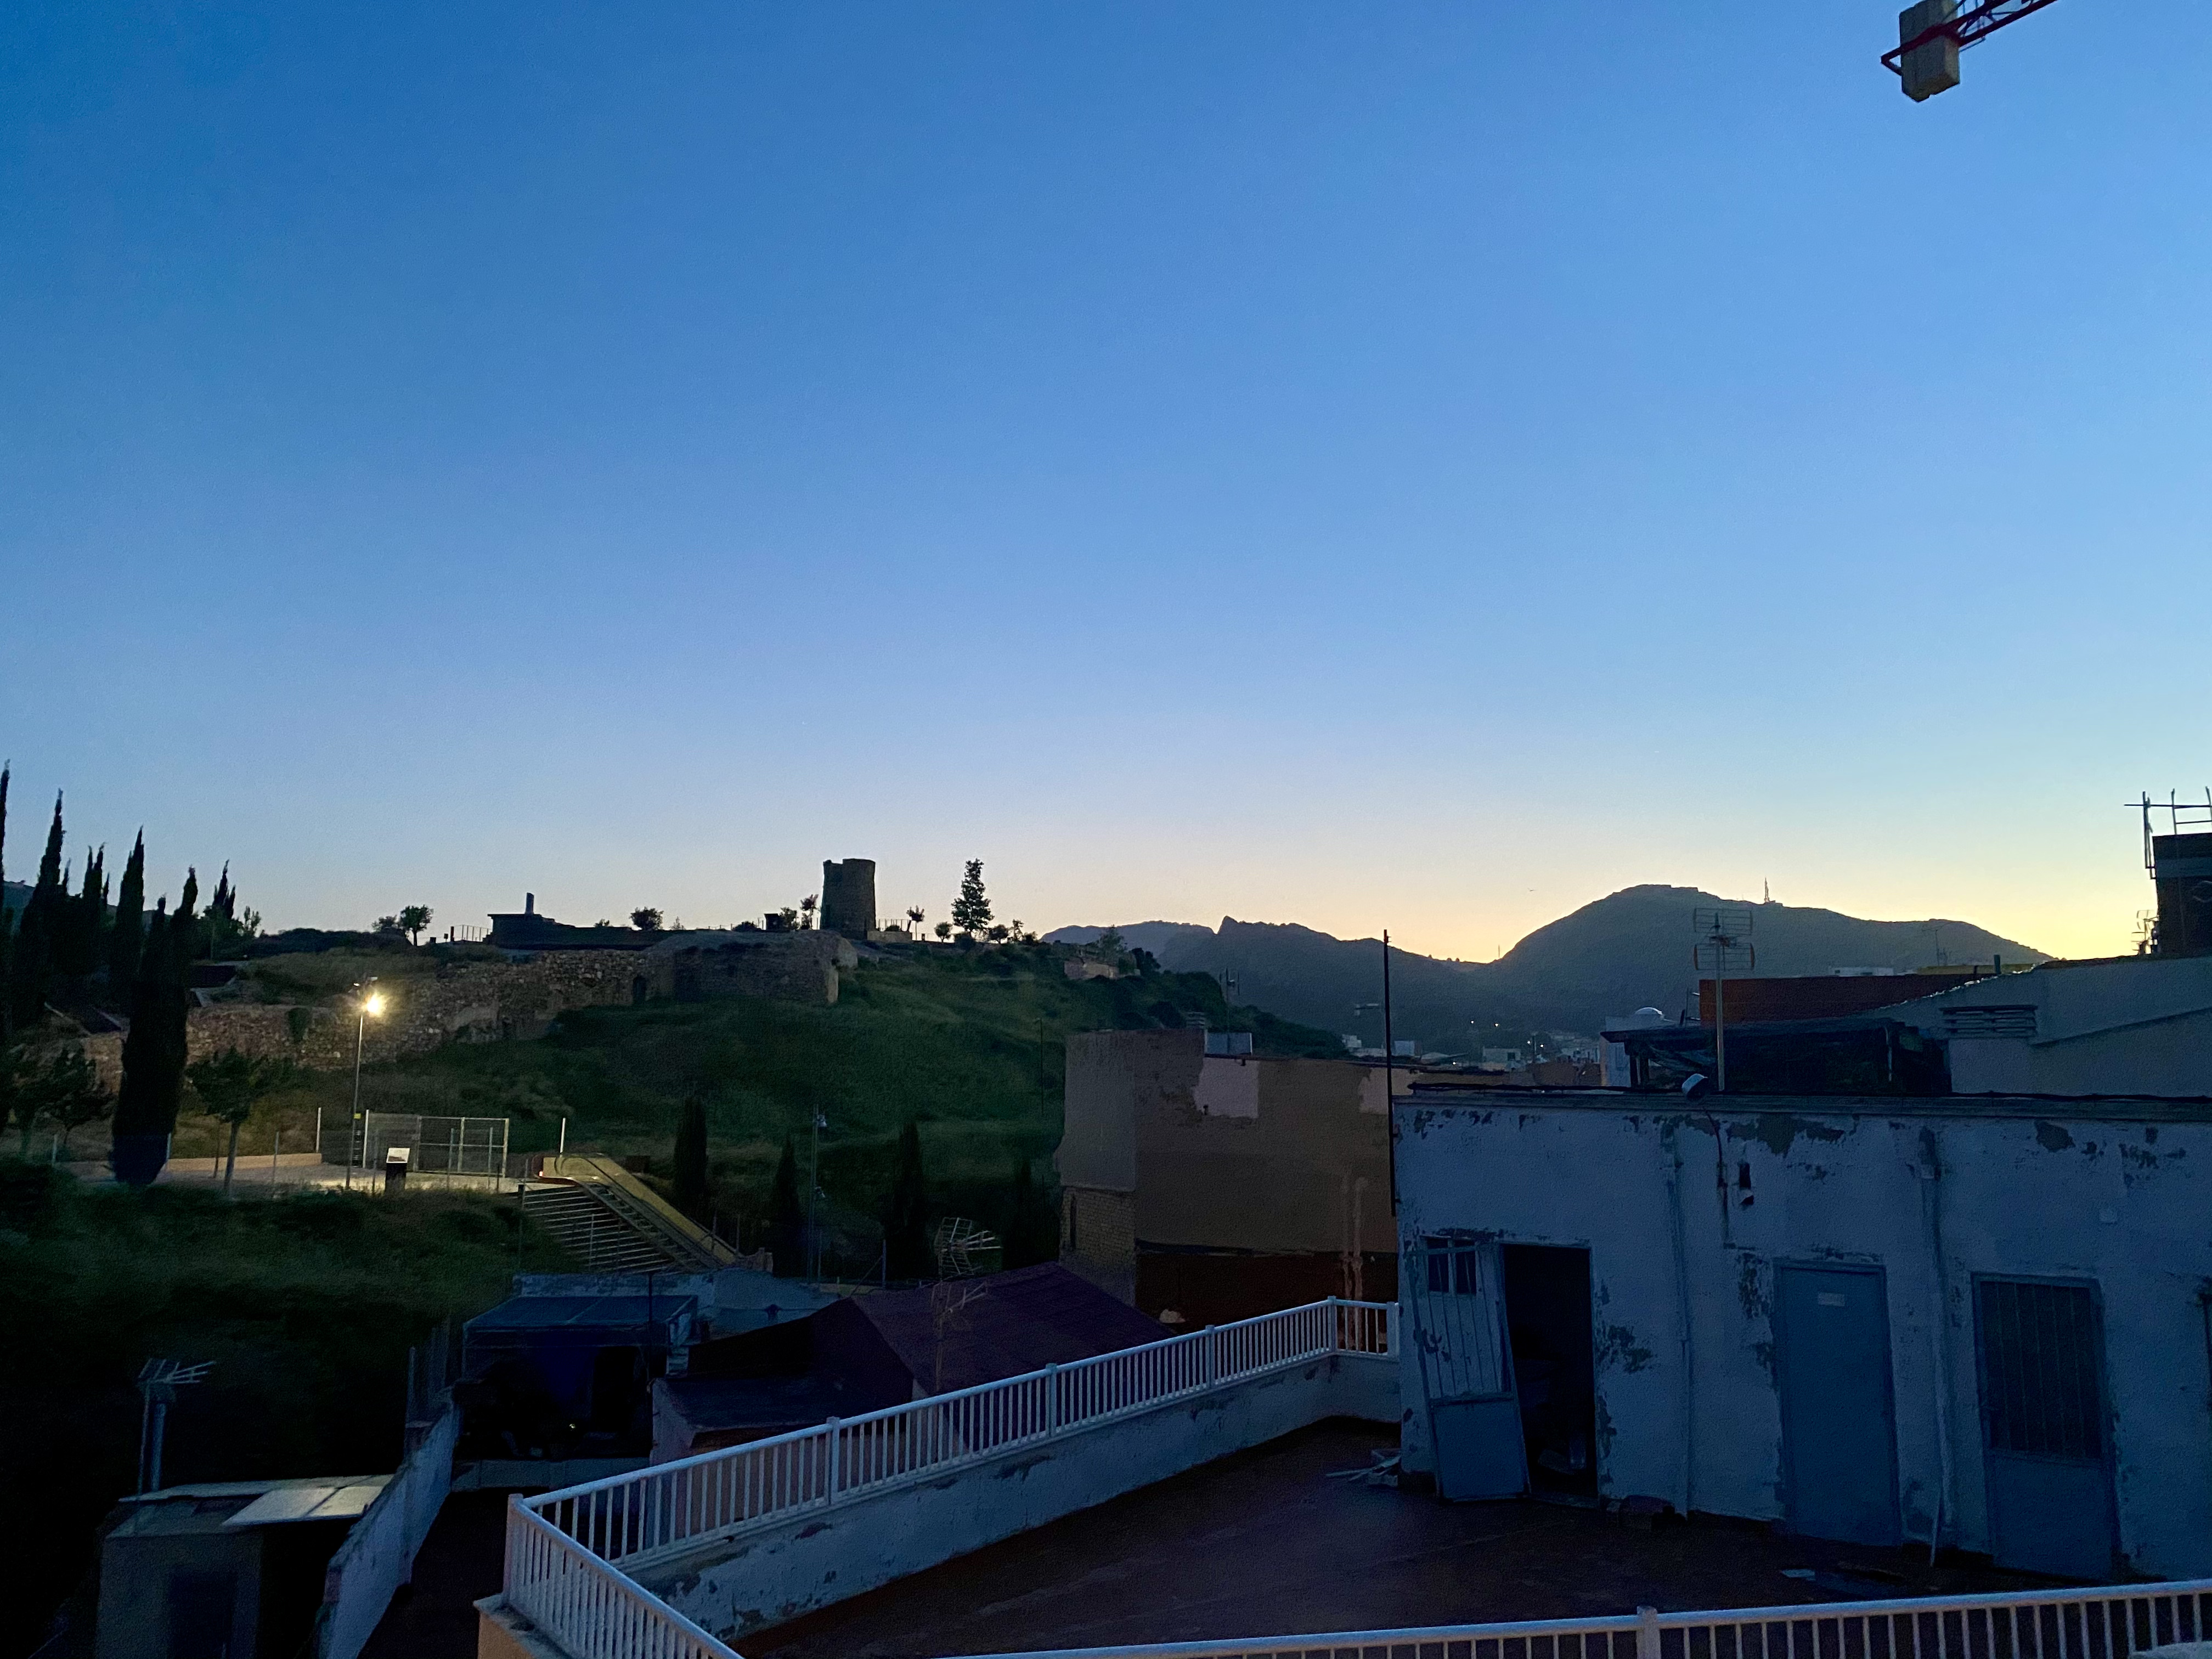
\includegraphics[width=10cm]{rooftop.jpeg}
\caption{Rooftop where the idea came to be}\label{rooftop}
\end{figure}

\subsection{Problem}
Suppose we have a load located at the starting location $S = (s_1,s_2)$ and its destination is the ending point $E = (e_1,e_2)$. The crane rotates at a constant angular velocity $\omega$ and starts rotating at time $t=0$ to the side of our choosing. The load carried by the crane can move along the arm of the crane and the speed along the arm is $c(t)$:

\begin{figure}[H]
\centering
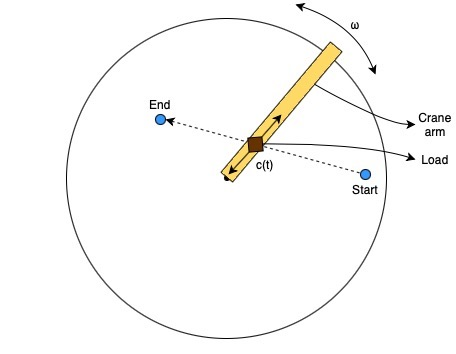
\includegraphics[width=10cm]{crane.jpg}
\caption{Crane - view from above}\label{crane}
\end{figure}

At time $t=0$ the load is located at the starting point and the crane immediately starts rotating such that it covers the smaller angle between starting and ending point. For example on the image above, the crane will rotate in the counter clockwise direction because both $S$ and $E$ are on the upper half of the circle. Had $E$ been in the lower half, the crane would start rotating in the clockwise direction. \\

\textbf{Problem:} Find the function $c(t)$ such that the load always has a linear trajectory from the start to the end (dashed line on the image above). For this problem there are no restrictions for the function $c(t)$ (such as maximum velocity or similar).

\section{Solution}

We can decompose the velocity of the load into 2 independent velocities: the velocity of the load caused by the rotation of the arm of the crane and the velocity of the load along the arm of the crane. First lets formally write down the velocity caused by the rotation of the arm.\\



\end{document}
